\documentclass[11pt]{article}
\usepackage[utf8]{inputenc}
\usepackage[spanish,es-nodecimaldot]{babel}
\usepackage[a4paper,margin=2.4cm]{geometry}
\usepackage{amsmath,booktabs,graphicx,siunitx,url}

\title{Test 5: Sensibilidad a malla y condiciones de borde en MEF 1D}
\author{Viviana Pérez Tapia}
\date{Noviembre 2026}

\begin{document}
\maketitle

\section{Problema y objetivo}
El objetivo de este trabajo es evaluar la sensibilidad del error de discretización espacial y la respuesta frente a condiciones de contorno cinemáticas en un modelo de elementos finitos unidimensional para una barra elástica lineal. Se analiza si la coincidencia exacta de desplazamientos nodales garantiza la precisión continua del campo en puntos intermedios, estudiando la tasa de convergencia para mallas de 2, 4 y 8 elementos. Asimismo, se evalúa el comportamiento del balance de reacciones al sobre-restringir el contorno con $u(L)=0$.

\section{Datos, supuestos y método}
Se modela una barra de longitud $L = \SI{2000}{\milli\metre}$, sección transversal $A = \SI{1000}{\square\milli\metre}$ y módulo elástico $E = \SI{200000}{\mega\pascal}$ ($EA = \SI{2e8}{\newton}$). La barra está empotrada en $x=0$ ($u(0)=0$), solicitada por una carga distribuida uniforme $q = \SI{10}{\newton\per\milli\metre}$ y una carga puntual en el extremo $P = \SI{20000}{\newton}$ aplicada en $x=L$. 

A partir de la ecuación diferencial de equilibrio elástico en barras, $-(EA u')' = q$, con condiciones $u(0)=0$ y $EA u'(L)=P$, la solución analítica exacta de referencia es:
\begin{equation}
u(x) = \frac{1}{EA}\left[(P + qL)x - \frac{1}{2}qx^2\right]
\label{eq:analitica}
\end{equation}
Evaluando en el extremo libre se obtiene teóricamente $u(L) = \SI{0.30}{\milli\metre}$ y una reacción $R_{\text{izq}} = -(P+qL) = \SI{-40000}{\newton}$. La resolución por MEF utiliza formulación de elementos lineales de dos nodos con interpolación isoparamétrica estándar y cálculo de vectores nodales consistentes \cite{zienkiewicz2005}. El error continuo se evalúa calculando el error absoluto máximo entre la solución aproximada lineal interpolada $u_h$ y la solución de referencia $u(x)$ en el punto medio de cada elemento.

\section{Resultados y verificación}
Las simulaciones ejecutadas mediante \texttt{src/ejecutar.py} arrojaron los resultados tabulados en el Cuadro~\ref{tab:resultados}. En todos los casos base, el equilibrio de fuerzas axiales se satisface de forma estricta con residuos del orden numérico de $10^{-11}\,\unit{\newton}$, cumpliendo la tolerancia relativa de máquina.

\begin{table}[htbp]
\centering
\small
\caption{Resultados numéricos MEF y evaluación de errores en puntos medios.}
\label{tab:resultados}
\begin{tabular}{lcccccc}
\toprule
Caso & $n$ & $u(L)$ [\unit{\milli\metre}] & $R_{\text{izq}}$ [\unit{\newton}] & $R_{\text{der}}$ [\unit{\newton}] & Error medio [\unit{\milli\metre}] & Balance [\unit{\newton}] \\
\midrule
M2 & 2 & 0.3000 & $-40000.0$ & 0.0 & \num{6.250e-3} & 0.0 \\
M4 & 4 & 0.3000 & $-40000.0$ & 0.0 & \num{1.562e-3} & \num{2.18e-11} \\
M8 & 8 & 0.3000 & $-40000.0$ & 0.0 & \num{3.906e-4} & \num{-3.64e-11} \\
BC\_ALTERADO & 8 & 0.0000 & $-10000.0$ & $-30000.0$ & --- & 0.0 \\
\bottomrule
\end{tabular}
\end{table}

\begin{figure}[htbp]
\centering
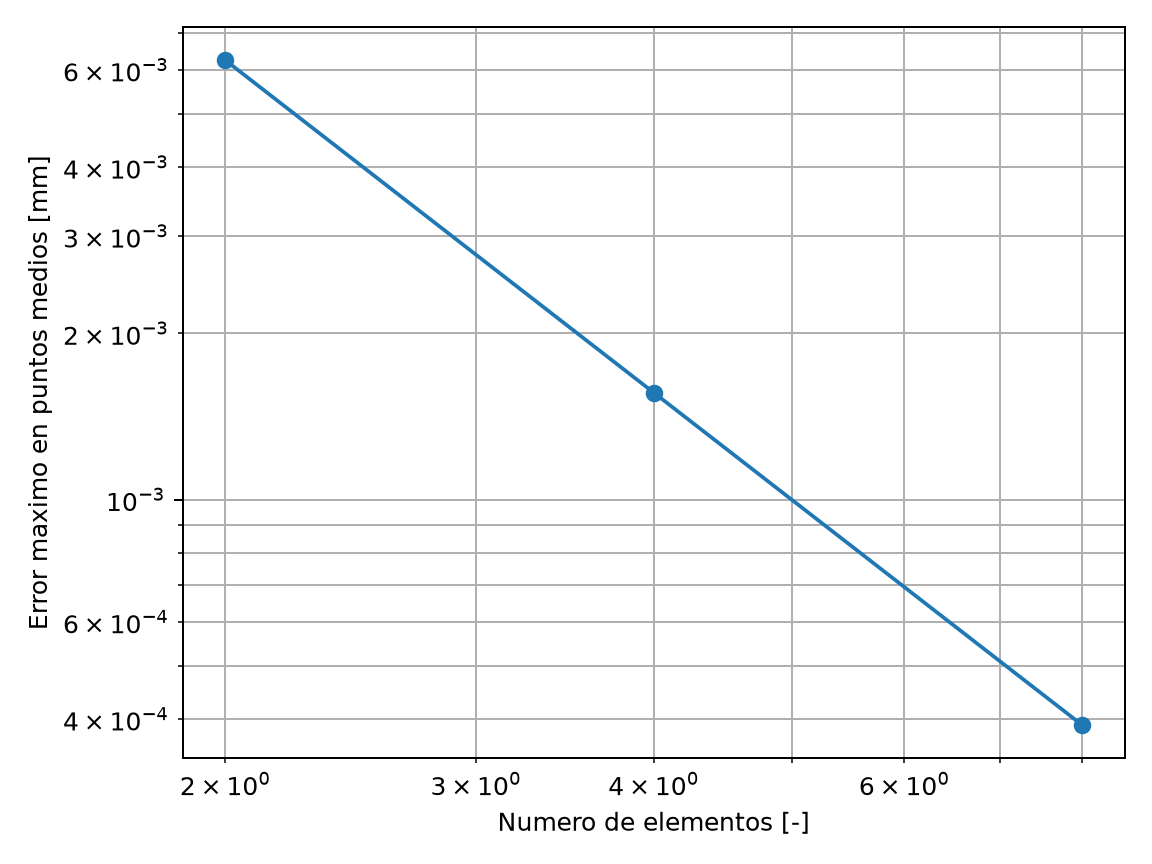
\includegraphics[width=0.60\textwidth]{../salidas/convergencia.png}
\caption{Curva de convergencia log-log del error máximo en puntos medios frente al número de elementos discretizados.}
\label{fig:convergencia}
\end{figure}

\section{Interpretación y conclusiones}
Para los modelos M2, M4 y M8 se comprueba el fenómeno de superconvergencia nodal en 1D: el desplazamiento en los nudos coincide de forma exacta con la solución analítica ($u(L)=\SI{0.30}{\milli\metre}$) sin importar el tamaño de malla. No obstante, al evaluar el campo continuo interior, se constata que la formulación lineal no capta la curvatura parabólica real de la barra entre nodos. El error máximo ocurre precisamente en los puntos medios y decae a razón cuadrática $\mathcal{O}(h^2)$, reduciéndose un factor de 4 al duplicar elementos (de $\SI{0.00625}{\milli\metre}$ a $\SI{0.00039}{\milli\metre}$). Por ende, la exactitud nodal no certifica la convergencia del campo interior.

En el caso BC\_ALTERADO ($u(L)=0$), el sistema pasa a ser una barra biempotrada estáticamente indeterminada. Aunque el equilibrio estático cierra numéricamente de forma exacta ($R_{\text{izq}} + R_{\text{der}} + qL + P = \SI{-10000}{\newton} - \SI{30000}{\newton} + \SI{20000}{\newton} + \SI{20000}{\newton} = 0$), el modelo representa un problema físico estructural completamente diferente al solicitado. La satisfacción del equilibrio numérico es una condición necesaria pero no suficiente para validar un modelo numérico.

\section*{Declaración de uso de IA}
Se empleó Gemini (noviembre 2026) como asistente técnico para deducir la solución analítica continua, estructurar el cálculo vectorial del error en puntos medios y formatear la presentación de datos en LaTeX. Todos los resultados y deducciones mecánicas fueron contrastados de forma manual mediante equilibrio estático y validados mediante la batería de pruebas \texttt{pytest}.

\bibliographystyle{plain}
\bibliography{referencias}

\end{document}
